%
% This is a borrowed LaTeX template file for lecture notes for CS267,
% Applications of Parallel Computing, UCBerkeley EECS Department.
% Now being used for CMU's 10725 Fall 2012 Optimization course
% taught by Geoff Gordon and Ryan Tibshirani.  When preparing 
% LaTeX notes for this class, please use this template.
%
% To familiarize yourself with this template, the body contains
% some examples of its use.  Look them over.  Then you can
% run LaTeX on this file.  After you have LaTeXed this file then
% you can look over the result either by printing it out with
% dvips or using xdvi. "pdflatex template.tex" should also work.
%

\documentclass[twoside]{article}
\setlength{\oddsidemargin}{0.25 in}
\setlength{\evensidemargin}{-0.25 in}
\setlength{\topmargin}{-0.6 in}
\setlength{\textwidth}{6.5 in}
\setlength{\textheight}{8.5 in}
\setlength{\headsep}{0.75 in}
\setlength{\parindent}{0 in}
\setlength{\parskip}{0.1 in}

%
% ADD PACKAGES here:
%

\usepackage{amsmath,amsfonts,graphicx}
\usepackage{enumitem}
\usepackage{verbatim}

%
% The following commands set up the lecnum (lecture number)
% counter and make various numbering schemes work relative
% to the lecture number.
%
\newcounter{lecnum}
\renewcommand{\thepage}{\thelecnum-\arabic{page}}
\renewcommand{\thesection}{\thelecnum.\arabic{section}}
\renewcommand{\theequation}{\thelecnum.\arabic{equation}}
\renewcommand{\thefigure}{\thelecnum.\arabic{figure}}
\renewcommand{\thetable}{\thelecnum.\arabic{table}}

%
% The following macro is used to generate the header.
%
\newcommand{\lecture}[4]{
   \pagestyle{myheadings}
   \thispagestyle{plain}
   \newpage
   \setcounter{lecnum}{#1}
   \setcounter{page}{1}
   \noindent
   \begin{center}
   \framebox{
      \vbox{\vspace{2mm}
    \hbox to 6.28in { {\bf UCSB CS 291D: Blockchains and Cryptocurrencies
	\hfill Fall 2020} }
       \vspace{4mm}
       \hbox to 6.28in { {\Large \hfill Lecture #1: #2  \hfill} }
       \vspace{2mm}
       \hbox to 6.28in { {\it Lecturer: #3 \hfill Scribes: #4} }
      \vspace{2mm}}
   }
   \end{center}
   \markboth{Lecture #1: #2}{Lecture #1: #2}

%   {\bf Note}: {\it LaTeX template courtesy of UC Berkeley EECS dept.}

%   {\bf Disclaimer}: {\it These notes have not been subjected to the
%   usual scrutiny reserved for formal publications.  They may be distributed
%   outside this class only with the permission of the Instructor.}
%   \vspace*{4mm}
}
%
% Convention for citations is authors' initials followed by the year.
% For example, to cite a paper by Leighton and Maggs you would type
% \cite{LM89}, and to cite a paper by Strassen you would type \cite{S69}.
% (To avoid bibliography problems, for now we redefine the \cite command.)
% Also commands that create a suitable format for the reference list.
\renewcommand{\cite}[1]{[#1]}
\def\beginrefs{\begin{list}%
        {[\arabic{equation}]}{\usecounter{equation}
         \setlength{\leftmargin}{2.0truecm}\setlength{\labelsep}{0.4truecm}%
         \setlength{\labelwidth}{1.6truecm}}}
\def\endrefs{\end{list}}
\def\bibentry#1{\item[\hbox{[#1]}]}

%Use this command for a figure; it puts a figure in wherever you want it.
%usage: \fig{NUMBER}{SPACE-IN-INCHES}{CAPTION}
\newcommand{\fig}[3]{
			\vspace{#2}
			\begin{center}
			Figure \thelecnum.#1:~#3
			\end{center}
	}
% Use these for theorems, lemmas, proofs, etc.
\newtheorem{theorem}{Theorem}[lecnum]
\newtheorem{lemma}[theorem]{Lemma}
\newtheorem{proposition}[theorem]{Proposition}
\newtheorem{claim}[theorem]{Claim}
\newtheorem{corollary}[theorem]{Corollary}
\newtheorem{definition}[theorem]{Definition}
\newenvironment{proof}{{\bf Proof:}}{\hfill\rule{2mm}{2mm}}

% **** IF YOU WANT TO DEFINE ADDITIONAL MACROS FOR YOURSELF, PUT THEM HERE:

\newcommand\E{\mathbb{E}}

\begin{document}
%FILL IN THE RIGHT INFO.
%\lecture{**LECTURE-TITLE**}{**DATE**}{**LECTURER**}{**SCRIBE**}
\lecture{11}{ZkSnark Internals}{Shumo Chu}{Sabrina Tsui, Abtin Bateni}
%\footnotetext{These notes are partially based on those of Nigel Mansell.}

% **** YOUR NOTES GO HERE:

% Some general latex examples and examples making use of the
% macros follow.  
%**** IN GENERAL, BE BRIEF. LONG SCRIBE NOTES, NO MATTER HOW WELL WRITTEN,
%**** ARE NEVER READ BY ANYBODY.

\section{Introduction} 
Last lecture, we discussed an introduction to ZkSnark, which is zero-knowledge succinct non-interactive argument of knowledge. This lecture builds on that introduction, namely exploring the ingredients necessary to understand how ZkSnark works under the hood. Although if you want to just use the ZkSnark you do not have to know this, this will hugely contribute to understanding and working with ZkSnark better.
\subsection{ZkSnark Pipeline}
This sections gives an overview of ZkSnark and is a recap to what we learned during the previous lecture. ZkSnark can prove any NP-statement. If you can demonstrate your statement in high level language (e.g. C/Python), as long as it does not have recursion you can use ZkSnark to prove it. The procedure first converts your program to an algebraic circuit and then, uses RICS (Rank 1 constraints system) followed by QAP(quadratic arithmetic program) and Linear PCP (probabilistic checkable proofs) and Linear Interactive proof. Finally, we use ZkSnark to finalize the proof.\\ \\
\textbf{Pipeline:}
\begin{enumerate}[topsep=0pt,itemsep=-1ex,partopsep=1ex,parsep=1ex]
    \item NP Statement
    \item Computation (high level language, i.e. C program)
    \item Algebraic circuit
    \item RICS (Rank 1 constraints system)
    \item QAP (quadratic arithmetic program)
    \item Linear PCP (probabilistic checkable proofs)
    \item ZkSnark
\end{enumerate}
\section{Polynomials}
In order to delve into ZkSnark we need some background in polynomials and in this section we are going to provide a background on the following terms.
\begin{enumerate}[topsep=0pt,itemsep=-1ex,partopsep=1ex,parsep=1ex]
    \item Homomorphic Hidings
    \item Blind Evaluation of Polynomials
    \item The knowledge of Coefficient Test and Assumptions
    \item Make Blind Evaluation of Polynomials Verifiable
\end{enumerate}
\subsection{Homomorphic Hiding}
A Homomorphic Hiding(HH) $E(x)$ of a number $x \in F_p$ is a function that satisfies:
\begin{enumerate}[topsep=0pt,itemsep=-1ex,partopsep=1ex,parsep=1ex]
    \item For most $x$, given $E(x)$, it is hard to find $x$ (with overwhelming probability, a randomly-sampled $x$ has this property.)
    \item Different inputs lead to different outputs. if $x\neq y then, E(x)\neq E(y)$
    \item If someone knows $E(x)$ and $E(y)$, then they can generate $E(x+y)$
\end{enumerate}
Hence, Homomorphic Hiding is similar to Homomorphic Encryption except you do not need decrypt. In fact, HH is just a concept and is like an abstraction for many cryptographic functions. For example, if Alice wants to prove to Bob that she knows $x$ and $y$ such that their sum equals to $7$, she can provide Bob with $E(x)$ and $E(y)$ and Bob can compute $E(x+y)$ and compare it with $E(7)$.
\subsubsection{Construct HH}
The following is one of the simplest HH functions: 
$n: [N]$ and $p$ is a prime, $E(n) = A \% p$. Consequently, $a+b$ would be defined as $(a+b) \% p$ and $a*b$ would be defined as $(a*b) \% p$. Our first conclusion would be that the addition and the multiplication operations are closed. That is, the result of the addition or multiplication of any two numbers still belong to the range of the HH function.\\ \\
Consider a group $F_p$ s.t.:
\begin{enumerate}[topsep=0pt,itemsep=-1ex,partopsep=1ex,parsep=1ex]
    \item It is a cyclic group. There exists an operation $g$ s.t. if we apply it $p$ times, it will cover the domain of $F_p$ (i.e. $0, 1, ..., p-1$).
    \item The discrete log is hard: If p is sufficiently large, given an element $h$ in $F_p$, it is hard to find $a$ s.t. $g^a = h$.
    \item Exponent add up element multiplied: $g^a.g^b = g^{a+b}$ \\
\end{enumerate}
The operation $g$ in this example acts an HH function with $E(x)=g^x$.
Note that in practice, HH functions can be implemented with elliptic curves. (See figure 11.1), RSA, or other cryptoprimitives. \\
\begin{figure}
    \centering
    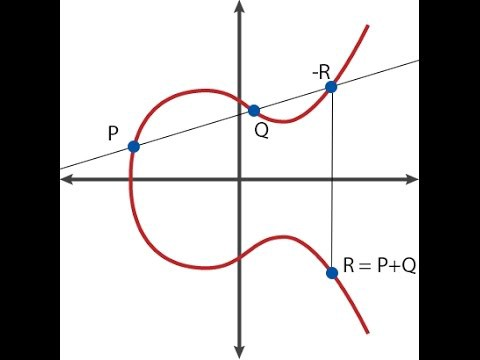
\includegraphics[scale=0.25]{elliptic1.jpg}
    \fig{1}{0.1in}{Elliptic Curve \cite{1}}
\end{figure}

\section{Blind Evaluation of Polynomials}
Consider the group $F_p$ defined in the previous section and the function $P$ s.t.:\\$P(X) = a_0 + a_1.X + a_2.X^2 + a_3.X^3 + ... + a_d.X^d$ and $a_0, a_1, ..., a_d \in F_p$\\
If $s \in F_p$, $P(s) = a_0*s^0 + a_1*s^1 + ... + a_d*s^d$. The function $P$ here acts as an HH function which also supports linear combination in addition to the addition and the multiplication operations (i.e. given $a$, $b$, $E(x)$, $E(y)$, we can compute $E(ax+by)$).\\
For example, if we consider the previously defined function $g$ as our HH function, then the following conclusion would arise. \\

Given a,b,E(x), and E(y), know E(ax+by). \\
E(x) = $g^x \Rightarrow E(ax+by) = g^{ax + by}$ \\
= $g^{ax} * g^{by}$ = $(g^x)^a * (g^y)^b$ \\
= $(E(x))^a * (E(y))^b$

For example, consider Alice has a polynomial $P$ with degree $d$ and Bob has random number $s \in F_p$. Bob wants to learn the value $E(P(s))$ but he should not know $P$ and Alice cannot learn the value $s$. To do so, Bob can send to Alice the values $E(s^0), E(s^1), ..., E(s^d)$. Since $P$ supports linear combination, Alice can compute $E(P(s))$ without learning $s$ from the previous values. Alice will finally send the result to Bob and the problem would be solved. However, this algorithms shows that Alice is aware of some polynomial $P$. Alice can change the polynomial each time and by using different polynomials can compromise Bob's assumptions. To tackle this problem, Bob can advantage of a process named The KC test.

\begin{comment}
\subsubsection{The KC test}
Consider $\alpha \in F_p$, $g$: generator of group $G$ which $|G|=p$. We call $(a, b)$ an $\alpha$-pair if $b=\alpha.a$. The algorithm is as follows:
\begin{enumerate}[topsep=0pt,itemsep=-1ex,partopsep=1ex,parsep=1ex]
    \item Bob chooses a random $\alpha \in F_p$ and $a \in G$ and computes $b=\alpha.a$
    \item Bob sends Alice the pair $(a, b)$
    \item Alice responses back with the pair $(a', b')$
    \item Bob checks whether $b' = \alpha.a'$
\end{enumerate}
This test shows that Alice is using an $\alpha$ and is not sending us totally random numbers.
\end{comment}


\begin{comment}
\section{Blind Evaluation of Polynomials}
The problem statement of blind evaluation of a polynomial is that Alice knows a polynomial P(x) with degree d. Suppose Bob wants to evaluate P(s) for a randomly generated s $\in$ $F_p$, with 2 conditions: Alice can't learn s, and Bob can compute E(P(s)) without knowing P. 
\subsection{Definition of Polynomial P(x)}
P(x) = $a_0 + a_1x + a_2x^2 + ... + a_dx^d$, where $a_0...a_d \in F_p$ are coefficients, and $x \in F_p$ is a variable. Recall $F_p = {0,1...p-1}$, p is prime. 
\subsection{Extend HH to support linear combinations}
Given a,b,E(x), and E(y), know E(ax+by). \\
E(x) = $g^x \Rightarrow E(ax+by) = g^{ax + by}$ \\
= $g^{ax} * g^{by}$ = $(g^x)^a * (g^y)^b$ \\
= $(E(x))^a * (E(y))^b$

$E(x) = g^x$, and $E(ax+by)=g^{ax+by}=g^{ax}.g^{by}=(g^x)^a.(g^y)^b=E(x)^a.E(y)^b$\\

\subsection{Protocol}
\begin{enumerate}
    \item Bob sends Alice $E(s^0) = E(1), E(s), E(s^2)...E(s^d)$. Note: it is not sufficient for Bob to simply send E(s) because of the discrete log problem. 
    \item Alice computes E(P(s)), which is a linear combination of coefficients $a_0...a_d$ and terms $s^0,s,s^2...s^d$.
    \item Alice sends computed value E(P(s)) to Bob.
\end{enumerate}
However, in this scheme, Bob cannot verify if Alice evaluated P(s) correctly!

\end{comment}

\section{The Knowledge of Coefficient Test}
The Knowledge of Coefficient test is used for a verifier (Bob) to know that a prover (Alice) knows some coefficient $\gamma$. This is useful in a later protocol that verifies Alice actually computes P(x) rather than some arbitrary polynomial, because P(x) contains coefficients $a_0...a_d \in F_p$. The protocol is explained below:
\begin{enumerate}
    \item Let $\alpha \in F_p$ and g be a generator of G, $|G| = P$. Define (a,b) is an $\alpha$-pair if b = $\alpha*a$. 
    \item Bob chooses a random $\alpha \in F_p$ and $a \in G$, then computes b = $\alpha * a$.
    \item Bob sends Alice (a,b) pair, but not $\alpha$. Only Bob knows $\alpha$. 
    \item Alice knows some value $\gamma$, so Alice computes a' = $\gamma a$, b' = $\gamma b$. Alice responds back (a', b'). 
    \item Bob checks if b' = $\alpha*a'$. (i.e. $g^{b'} = g^{\alpha a'}$). If the check passes (b' does equal $\alpha*a'$), with non-negligible probability, Alice knows a $\gamma$ such that a' = $\gamma$a
\end{enumerate}

\section*{References}
\beginrefs
\bibentry{1}{\sc Extropy.io}, 
``Maths Primer for Zero Knowledge Workshop,'' \\
{\it http://extropy.foundation/workshops/zkp/primer.html}
\endrefs



% **** THIS ENDS THE EXAMPLES. DON'T DELETE THE FOLLOWING LINE:

\end{document}





\begin{comment}

\subsection{Code from the template for reference - delete if not needed}
We now delve right into the proof.

\begin{lemma}
This is the first lemma of the lecture.
\end{lemma}

\begin{proof}
The proof is by induction on $\ldots$.
For fun, we throw in a figure.
%%%NOTE USAGE !
\fig{1}{1in}{A Fun Figure}

This is the end of the proof, which is marked with a little box.
\end{proof}

\subsection{A few items of note}

Here is an itemized list:
\begin{itemize}
\item this is the first item;
\item this is the second item.
\end{itemize}

Here is an enumerated list:
\begin{enumerate}
\item this is the first item;
\item this is the second item.
\end{enumerate}

Here is an exercise:

{\bf Exercise:}  Show that ${\rm P}\ne{\rm NP}$.

Here is how to define things in the proper mathematical style.
Let $f_k$ be the $AND-OR$ function, defined by

\[ f_k(x_1, x_2, \ldots, x_{2^k}) = \left\{ \begin{array}{ll}

	x_1 & \mbox{if $k = 0$;} \\

	AND(f_{k-1}(x_1, \ldots, x_{2^{k-1}}),
	   f_{k-1}(x_{2^{k-1} + 1}, \ldots, x_{2^k}))
	 & \mbox{if $k$ is even;} \\

	OR(f_{k-1}(x_1, \ldots, x_{2^{k-1}}),
	   f_{k-1}(x_{2^{k-1} + 1}, \ldots, x_{2^k}))	
	& \mbox{otherwise.} 
	\end{array}
	\right. \]

\begin{theorem}
This is the first theorem.
\end{theorem}

\begin{proof}
This is the proof of the first theorem. We show how to write pseudo-code now.
%*** USE PSEUDO-CODE ONLY IF IT IS CLEARER THAN AN ENGLISH DESCRIPTION

Consider a comparison between $x$ and~$y$:
\begin{tabbing}
\hspace*{.25in} \= \hspace*{.25in} \= \hspace*{.25in} \= \hspace*{.25in} \= \hspace*{.25in} \=\kill
\>{\bf if} $x$ or $y$ or both are in $S$ {\bf then } \\
\>\> answer accordingly \\
\>{\bf else} \\
\>\>    Make the element with the larger score (say $x$) win the comparison \\
\>\> {\bf if} $F(x) + F(y) < \frac{n}{t-1}$ {\bf then} \\%
\>\>\> $F(x) \leftarrow F(x) + F(y)$ \\
\>\>\> $F(y) \leftarrow 0$ \\
\>\> {\bf else}  \\
\>\>\> $S \leftarrow S \cup \{ x \} $ \\
\>\>\> $r \leftarrow r+1$ \\
\>\> {\bf endif} \\
\>{\bf endif} 
\end{tabbing}

This concludes the proof.
\end{proof}
Here is a citation, just for fun~\cite{CW87}.


\end{comment}


